\section{Theorie}
\label{sec:theorie}
In diesem Teil des Protokoll werden die theoretischen Grundlagen des Versuchs erarbeitet.
\subsection{Das Myon}
Myonen sind leptonische Elementarteilchen.
Sie werden in das Standardmodell zwischen den Elektronen und den Tauonen eingeordnet und besitzen eine Masse von $m_\mu = \SI{105.65}{\mega\eV}$ \cite{myonen}.
Sie sind genauso wie das Elektronen negativ geladen, wobei diese Ladung betragsmäßig einer Elementarladung $e$ entspricht.
Im Gegensatz zum Elektronen zerfallen Myonen allerdings nach kurzer Zeit, ihre mittlere Lebenszeit beträgt dabei $\tau_\mu = \SI{2.196}{\micro\second}$ \cite{myonen}.
\subsubsection{Kosmische Myonen}
Die Quelle von Myonen die in diesem Versuch verwendet wird, sind kosmische Myonen.
Diese entstehen als Teil einer Zerfallskette, welche durch ein Proton ausgelöst wird.
Die Protonen stammen dabei zum größten Teil von der Sonne.\\
Wenn das Proton in die Erdatmosphäre eintritt löst dieses einen hadronischen Schauer aus.
Dabei zerfällt das Proton am häufigsten in ein Pion $\pi$.
Ein Zerfall in ein Kaon $K$ ist auch möglich, tritt allerdings nur in $(10-15)\%$ der Fälle auf.
\FloatBarrier
\begin{figure}
    \begin{minipage}{0.55\textwidth}
Die entstanden Pionen können entweder neutral $\pi^0$ oder geladen $\pi+$, $\pi-$ sein.
Die neutralen Pionen zerfallen dabei wesentlich schneller als die Ungeladenen und lösen durch ihren Zerfall eine elektromagnetische Kaskade aus $(\pi^0 \rightarrow \gamma +\gamma)$ aus.
Diese Schauerkomponente ist für uns nur von geringer Bedeutung, da die Kaskade meist noch in der Atmosphäre endet.\\
Geladene Pionen haben eine längere Lebenszeit und zerfallen in einer Höhe von ungefähr $\SI{10}{\kilo\meter}$.
Durch ihre Zerfälle entstehen Myonen die in diesem Versuch gemessen werden sollen.
Die Zerfälle sehen wie folgt aus:\\ $\pi-\rightarrow \mu^- +\bar{\nu_\mu}$, also ein negatives Pionen zerfällt in ein Myon und ein Antineutrino,\\ oder $\pi+\rightarrow \mu^+ + \nu_\mu$, also ein positiv geladenes Pion zerfällt in ein Antimyon und ein Neutrino.
Die gesamte Zerfallskette wird in Abbildung \ref{fig:hadronischerschauer} veranschaulicht.
\end{minipage}
\hfill
\begin{minipage}{0.4\textwidth}
    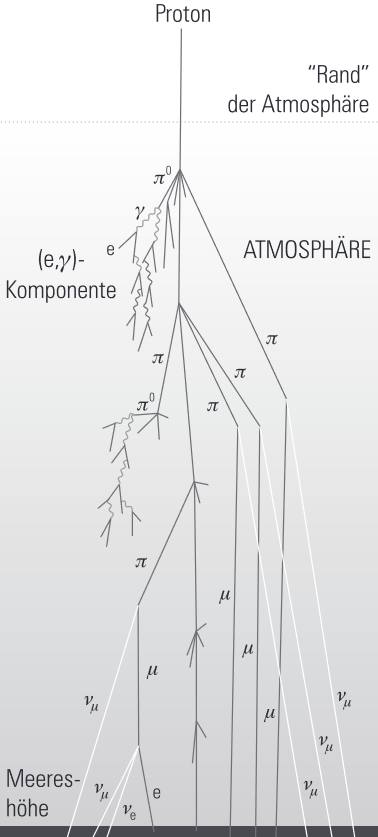
\includegraphics[width=\textwidth]{data/hadronischerschauer.png}
    \caption{Ein statischer hadronischer Schauer, welcher durch ein Proton ausgelöst wird.
    Es werden die möglichen Zerfallsketten dargestellt die bei einem solchen Schauer auftreten können. \cite{astroteilchenbuch}}
    \label{fig:hadronischerschauer}
\end{minipage}
\end{figure}\FloatBarrier
Es fällt nun auf, dass trotz der hohen Geschwindigkeit der entstandenen Myonen von $0.999c$ mit $c$ als Lichtgeschwindigkeit im Vakuum, die Myonen nicht auf der Erde ankommen sollten.
Denn sie würden aufgrund ihrer kurzen Lebensdauer nach ungefähr $\SI{650}{\meter}$ zerfallen, also bevor sie die Erdoberfläche erreichen.
Dies gilt allerdings nur für die klassische Betrachtung.\\
Da das Myon aber eine hoch relativistische Geschwindigkeit besitzt, tritt im Bezugssystem des Myons Längenkontraktion auf.
Wenn dieser relativistische Effekt beachtet wird, ändert sich die Flugdistanz des Myons auf $\SI{62}{\kilo\meter}$. \\
Da das Myon eine relativistische Geschwindigkeit besitzt ist es sehr unwahrscheinlich, dass es, ohne weitere Effekte zu nutzen, in der Detektorkammer zerfällt.
Aus diesem Grund wird ein Szintillator genutzt.
In diesem deponiert das Myon sehr viel Energie und wird so gebremst. 
So steigt die Rate an Myonen die tatsächlich im Szintillator zerfallen und keine Fehlmessung auslösen.
\subsection{Zerfallszeit}
Die Anzahl von Myonen $\symup{d}N$ die in einem Zeitintervall $\symup{d}t$ im Tank zerfallen, ist gegeben durch die Differentialgleichung
\begin{equation*}
    \symup{d}N = -\lambda N \symup{d}t\, ,
\end{equation*}
wobei $\lambda$ die Zerfallskonstante ist.
Diese Differentialgleichung wird durch den Ansatz 
\begin{equation}
    N(t) = N_0 \exp(-\lambda t)
    \label{eq:zerfall}
\end{equation}
gelöst, wobei $N_0$ die Anzahl der Teilchen zum Zeitpunkt $t=0$ ist.
Durch Gleichung \eqref{eq:zerfall} kann anschließend die mittlere Lebensdauer $\lambda = 1/\tau$ bestimmt werden.
\subsection{Untergrund}
Die Messung leidet unter einem Poisson verteilten Untergrund.
Sein Ursprung liegt darin, dass ein zweites Myon in die Detektorkammer eintreten kann.
Dieses Eintreten würde die Messung der Zerfallszeit des ersten Myons unterbrechen.
Um den Effekt durch den Untergrund so gering wie möglich zu halten, wird die theoretische Untergrundrate berechnet.
Die Anzahl der gemessenen Myonen $n$ folgt der Poissonverteilung
\begin{equation*}
    p(n) = \frac{\lambda^n}{n!} \exp(-\lambda)\, ,
\end{equation*}
hier ist $\lambda$ der Erwartungswert der Verteilung, welcher durch 
\begin{equation*}
    \lambda = \frac{N_\text{ges}}{t_\text{ges}} T_\text{such}
\end{equation*}
gegeben ist.
Dabei entspricht $N_\text{ges}$ der gesamt Anzahl an detektierten Eintrittsimpulsen in dem Messintervall $t_\text{ges}$.
Die Suchzeit $T_\text{such}$ ist die Zeit in der der Detektor aktiv bleibt.
Sollte der Detektor in der Zeit $T_\text{such}$ keinen zweiten Impuls, also optimalerweise einen Zerfallsimpuls, messen, wird die Messung verworfen.
Der Untergrund ergibt sich aus 
\begin{equation}
    U(N_\text{ges}) = N_\text{ges} p(1)\, ,
    \label{eq:untergrund}
\end{equation}
wobei $p(1)$ die Wahrscheinlichkeit dafür ist, dass während der Suchzeit nur genau ein Myon in die Detektorkammer fällt.